\chapter{Teoremi di convergenza}
\section{Verso la statistica}
Introduciamo ora un modello probabilistico fondamentale per la \textbf{statistica}:
\begin{center}
    Successione $X_1,X_2,X_3,...$ di Variabili Aleatorie
    \\\textbf{I.I.D} = Indipendenti e Identicamente Distribuite\footnote{Con la stessa distribuzione.}.
\end{center}
Concretamente, le variabili $X_i$ possono rappresentare misure o rilevazioni indipendenti, ripetute nel tempo di una sterssa quantità che si vuole studiare.
Tipicamente, queste varibili sono:
\begin{itemize}
    \item Discrete, con la stessa densità discreta fissata: $ \rightarrow p_{X_i}(x) = p(x) $
    \item Assolutamente continue, con la stessa densità fissata: $ \rightarrow f_{x_i} (x) = f(x)$
\end{itemize}
\esempio{Lancio ripetutamente un dado a sei faccie:
    \begin{center}
        $X_i:=$ Risultato del lancio $i$-esimo
    \end{center}
}
\esempio{Rilevo la pressione arteriosa in un campione di pazienti:
    \begin{center}
        $X_i:=$ valore della pressione misurata nel paziente $i$-esimo
    \end{center}
}

\paragraph{Problema} $p(x), f(x)$ non sono completamente note, come faccio quindi a trovare la distribuzione comune delle variabili?
Uso al Statistica Inferenziale.
\section{Statistica Inferenziale} 
Dalle osservazioni posso fare delle deduzioni, ovvero delle Inferenze, sulla distribuzione
comune di $X_1, X_2$ ossia su $p(x)$ e $f(x)$.

Non sempre posso osservare tutte le V.A e per questo ne scelgo casualmente $n$ formando un campione: 
\begin{center}
    $X_1, \dots ,X_n$ è  \textbf{Campione Aleatorio} di ampiezza $n$ $\to n$ V.A. I.I.D. 
\end{center}
Noi lavoreremo con variabili aleatorie che siano funzioni del 
campione aleatorio, cioè del tipo $g(x_1, \dots ,X_n)$:
\definizione{
    Dato un campione aleatorio $X_1, \dots, X_n$ una \textbf{Statistica Campionaria}
    è una qualunque funzione del campione:
    \[
        g(X_1, \dots, X_n) \text{   } (g:\mathbb{R}^n\rightarrow\mathbb{R})
    \]
}

% \paragraph*{Esempio di statistica campionaria} Media campionaria
% \begin{equation*}
%     \bar{X_n}:\frac{1}{n}\sum_{n=1}^n X_i
% \end{equation*}
Se $X_1,...,X_n$ sono variabili I.I.D. di media $\mu$ e varianza $\sigma^2$, allora:
\[ E[X_i] = \mu \;\;\; var(X_i) = \sigma^2 \]
\[ \to E(\bar{X}_n) = \mu  \;\;\; var(\bar{X}_n) = \frac{\sigma^2}{n} \]


\section{Legge dei Grandi Numeri}
Siano $X_1,X_2,...$ Variabili Aleatorie reali indipendenti e identicamente distribuite.
\\Sia $\mu = E[X_i]$, $\sigma^2 = Var[X_i]$
\osservazione{Siccome le variabili sono identicamente distribuite, $\mu$ e $\sigma^2$ sono uguali per ogni variabile.}

Introduciamo la \textbf{Media Campionaria}:
\[ \bar{X}_N  := \frac{1}{N} \sum_{i=1}^N X_i = \frac{X_1+X_2+ ... + X_N}{N}\]
Questa è una \emph{nuova variabile aleatoria} distinta dalle $X_i$.

Possiamo ora introdurre la legge dei grandi numeri:
\teorema[Legge dei Grandi Numeri]{
    Per ogni $\epsilon > 0$ avremo che:
    \[ \lim_{N\to\infty} P(|\bar{X}_N - \mu | \geq \epsilon ) = 0\]
    \[ \Longleftrightarrow \lim_{N\to\infty} P(\bar{X}_N \in (\mu - \epsilon, \mu + \epsilon)) = 1 \] 
}
A partire dalla sequenza di dati osservati $X_1,X_2,...,X_N$, posso essere fiducioso che la media dei dati
$\bar{X}$ sia vicina a $\mu = E[X]$, e che la distribuzione di $\bar{X}_n$ è concentrata attorno alla media $\mu$.

\osservazione{La Legge dei Grandi Numeri implica che il legame tra media campionaria e media $=$ valore atteso di $\mu$.}

La legge dei grandi numeri si dimostra con la \textbf{disuguaglianza di Chebishev}.
%\subsection{Dimostrazione della legge dei grandi numeri}
%Pagina 18, lezione 8.

\section{Distribuzione di X}
\begin{equation*}
    \mathbb{P} (a  < \bar{X_nx} \leq b) = \mathbb{P} (\frac{a - \mu}{\frac{\sigma}{\sqrt{n}}} 
    < \frac{X_n - \mu}{\frac{\sigma}{\sqrt{n}}} \leq \frac{b - \mu}{\frac{\sigma}{\sqrt{n}}})   
\end{equation*}
\begin{equation*}
    \text{Var}(\bar{X_n}) = \frac{\sigma ^ 2}{n} 
\end{equation*}
\begin{equation*}
    \frac{\sigma}{\sqrt{n}} = \sqrt{\text{Var}}
\end{equation*}



\section{Teorema del limite centrale}
Siano $X_1, ..., X_n$ v.a i.i.d. (Variabili aleatorie indipendenti identicamente distribuite)
$E(i) = \mu$ e $\text{Var}X_i = \sigma^2$ (con media e varianza finite).
\begin{equation*}
    \mathbb{P} (\frac{X_n-\mu}{\frac{\sigma}{\sqrt{n}}} \leq t) \rightarrow \Phi (t) \quad n \rightarrow + \infty   
\end{equation*}
Dove $\Phi$ è la funzione di ripartizione di una V.A $Z\sim N(0,1)$
\begin{equation*}
    \Phi(t) = \mathbb{P}(Z \leq t)
\end{equation*}
\paragraph*{Condizione per usare l'approssimazione normale} Abbiamo definito 
che solo con $n \geq 30$ si può usare l'approx per semplicità, in realtà non è semplice
dare un criterio univoco dato che dipende dall'asimmetria del campione di partenza.
\paragraph*{Nota per i campioni discreti} Quando ho un campione discreto è sempre necessario
applicare la correzione di continuità 
%https://it.wikipedia.org/wiki/Standardizzazione_(statistica)

\section*{Note per esercizi}
\begin{itemize}
    \item Riconosci la distribuzione notevole
    \item Ricava media e Var
    \item Scrivi la formula che ti serve (es P che una va sia $\leq$ di n)
    \item Effettua la correzione di continuità se si tratta di una VA discreta
    \item Verifica se $n\geq 30$, questo per verificare se si può applicare il TLC (teorema del limite centrale)
    \item Sottrai media e dividi per $\sqrt{\text{Var}}$
    \item Se hai $>$ come segno, anzichè $\mathbb{P}$ dovrai trovare $1-\mathbb{P}$ e invertire il segno in $<$
    \item Se trovi un valore $z$ negativo all'interno di $\Phi(z)$ dovrai calcolare $1 - \Phi(-z)$, quindi rendere positivo
    z, calcolare il suo $\Phi$ e sottrarlo a 1
\end{itemize}

\pagebreak
\section{Le Domande di Teoria}
Di seguito riporto alcune domande di teoria sui teoremi di convergenza:
\paragraph{Domanda 1}
\begin{center}
    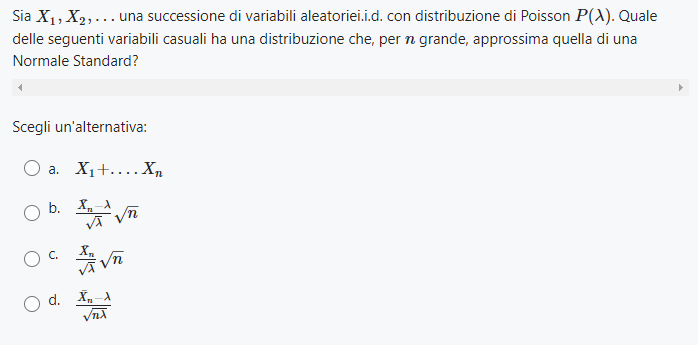
\includegraphics[width=.8\textwidth]{domanda4-1.png}
\end{center}
